\section{Abläufe}

Während in Kapitel 2 die Interaktion der Hauptkomponenten Server und der RobotUnit bzw. möglichen Kunden abgehandelt wurden, werden im Folgenden die Abläufe der innerhalb der Pakete genauer spezifiziert und auch interne Komponentenabläufe beschrieben.

\subsection*{Interaktion bei Ausführung von \textit{chooseRobot}}


\begin{figure}[H]
	\centering
	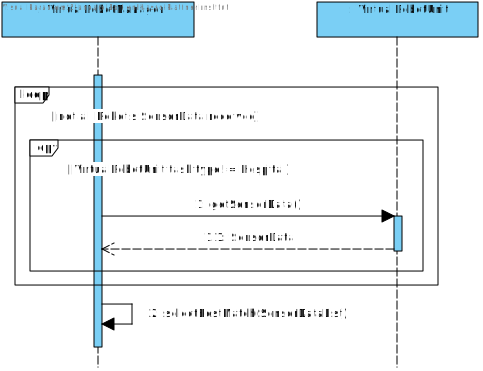
\includegraphics[width=1\textwidth]{img/8-chooseRobot}
	\caption{Sequenzdiagramm von \emph{chooseRobot}}
	\label{chooseRobotInteraktion}
\end{figure}
In der Hauptklasse \textit{VirtualRobotManager} der \textit{ServerSoftware} wird dieser Ablauf ausgeführt, wenn der zu einem zu verteilnden \textit{Task} am besten passendste \textit{VirtualRobotUnit} bzw. der dazugehörige \textit{Robot} ermittelt werden soll. Dabei werden Sensordaten von jedem \textit{Robot}, der nicht gerade einen Krankenhaustransport ausführt, gesammelt. Diese werden anschließend in der Methode \texttt{selectBestMatch} ausgewertet.
\\

\subsection*{Interaktion bei Ausführung von \textit{readSensors}}


\begin{figure}[H]
	\centering
	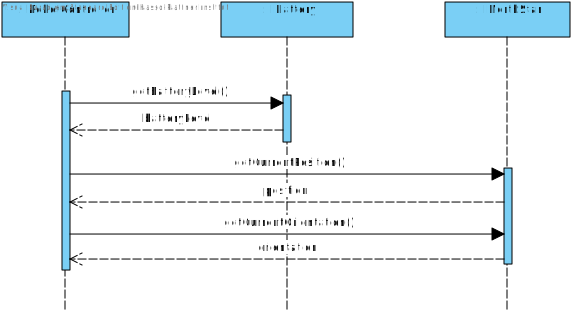
\includegraphics[width=1\textwidth]{img/8-readSensor}
	\caption{Sequenzdiagramm von \emph{readSensors}}
	\label{ReadSensorsInteraktion}
\end{figure}
Diese Interaktion ensteht innerhalb der \textit{RobotSoftware} in der Klasse \textit{RobotController} genau dann, wenn der \textit{Server} von allen \textit{Robots} im Rahmen von \texttt{getSensorData} die Sensordaten von allen  \textit{Robots} sammelt. Der \textit{RobotController} steuert dann die Hardware-Schnittstellen des \textit{Robots} an und sammelt die Sensordaten.
\\
	
\subsection*{Interaktion bei Ausführung von \textit{driveToDestination}}


\begin{figure}[H]
	\centering
	\includegraphics[width=1\textwidth]{img/8-driveToDestination}
	\caption{Sequenzdiagramm von \emph{8-DriveToDestination}}
	\label{driveToDestinationInteraktion}
\end{figure}
Diese Interaktion beschreibt die allgemeine Interaktion während des Anfahren eines Ziels innerhalb der \textit{RobotSoftware}. Genauer wird die Interaktion zwischen der im \textit{Robot} für das fahren zuständige \textit{DrivingSystem} und den Hardwareschnittstellen des \textit{Robots} modelliert. Der Vorgang wird duch einen möglichen Unfall unterbrochen.
\\

	
\subsection*{Interaktion bei Ausführung von \textit{requestRepair}}

\begin{figure}[H]
	\centering
	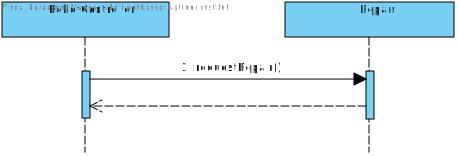
\includegraphics[width=1\textwidth]{img/8-requestRepair}
	\caption{Sequenzdiagramm von \emph{requestRepair}}
	\label{requestRepairInteraktion}
\end{figure}

Diese Interaktion entsteht dann, wenn ein \textit{Robot} verunglückt. Dabei wird durch den \textit{BumperHandler} ausgelöst, dass in der Hauptklasse \textit{RobotController} der \textit{RobotSoftware} über die von uns definierte Schnittstelle \textit{IRepair} der \textit{Server} über den Unfall benachrichtigt wird.\\
